\documentclass[11pt]{article}
\usepackage[utf8]{inputenc}
\usepackage[english]{babel}
\usepackage{amsfonts, amsmath, amssymb, amsthm}
\usepackage[none]{hyphenat}
\usepackage{fancyhdr}
\usepackage{graphicx}
\usepackage{float}
\usepackage{url}
\def\UrlBreaks{\do\/\do-}
\usepackage{breakurl}
\usepackage[breaklinks]{hyperref}
\usepackage[nottoc, notlot, notlof]{tocbibind}
\usepackage{algpseudocode}
\usepackage{mathtools}

\DeclarePairedDelimiter\floor{\lfloor}{\rfloor}

\theoremstyle{definition}
\newtheorem{definition}{Definition}[section]
\newtheorem{theorem}{Theorem}[section]
\newtheorem{lemma}{Lemma}[section]

\pagestyle{fancy}
\fancyhead{}
\fancyfoot{}
\fancyhead[L]{\slshape \MakeUppercase{High Performance Computing}}
\fancyhead[R]{\slshape \MakeUppercase{June 8, 2020}}
\fancyfoot[C]{\thepage}
\fancyfoot[R]{\slshape \MakeUppercase{Elie Saad}}
\renewcommand{\headrulewidth}{0pt}

\begin{document}

\begin{titlepage}
\begin{center}
\vspace*{1cm}
\Large{\textbf{\MakeUppercase{Warsaw University of Technology}}}\\[3mm]
\huge{\textbf{High Performance Computing}}\\[3mm]
\Large{\textbf{Faculty of Mathematics and Information Science}}\\
\vfill
\line(1,0){400}\\[1mm]
\huge{\textbf{Project 3}}\\[3mm]
\Large{\textbf{- Final Report -}}\\[1mm]
\line(1,0){400}\\
\vfill
By \textbf{Elie SAAD}\\
\Large{\textbf{June 8, 2020}}\\
\end{center}
\end{titlepage}

\tableofcontents
\thispagestyle{empty}
\clearpage

\section{Introduction}

\subsection{Problem Statement}

The following problem statement has been given:
\begin{center}
\textit{"Parallel ILLT for sparse symmetric matrix divided by columns. We remember only non-zeros of the matrix."}
\end{center}

\subsection{Problem Description}

Based on the problem statement above, we are required to consider the incomplete Cholesky factorizations (ILLT) for the iterative solution of sparse symmetric positive definite (SPD) $N\times N$ linear systems
\begin{equation*}
Au=b.
\end{equation*}
Incomplete Cholesky factorizations are commonly described with the help of Cholesky version of Gaussian elimination, which amounts to compute a lower triangular matrix $L$ such that $A=LL^T$ where $L$ is a factor of $A$ produced by exact elimination. Whereas the incomplete factorization is obtained by introducing approximation - or lack thereof - into the elimination process in an attempt to avoid non-zeros fill ins (non-zeros would replace the elements in $A$ where they themselves are zeros). Keeping the factors as close to being sparse like $A$, or as close to being dense like the factors computed by their exact elimination counterpart. This process is notably used as a preconditioner for an iterative method for a sparse SPD linear system. Thus, we are required to apply the ILLT algorithm, on a sparse SPD, over multiple processes.

\section{Definitions}

\begin{definition}[Positive Definiteness]
Let $A$ be an $n\times n$ matrix. $A$ is called a \textbf{positive definite} matrix if $x^TAx>0$ for every nonzero vector $x$ \cite{sympd}\cite{positivedefinite}.
\end{definition}

\begin{definition}[Symmetric Matrix]
Let $A$ be an $n\times n$ matrix. $A$ is called a \textbf{symmetric matrix} if and only if $A=A^T$ \cite{sympd}.
\end{definition}

\begin{definition}[Sparse Matrix]
A matrix where the majority of the values are zero is called a \textbf{sparse matrix}.
\end{definition}

\begin{definition}[Cholesky Factorization]
A symmetric positive definite $(n\times n)$-matrix $A$ can be decomposed as $A=R^TR$ where $R$, the Cholesky factor, is a upper triangular matrix with positive diagonal elements \cite{golub83matrix}. It can also be written as $A=LL^T$ where $L$ is the lower triangular matrix with positive diagonal elements. Both forms of the solution are unique.
\end{definition}

\begin{definition}[Preconditioners]
A \textbf{preconditioner} $P\approx A$ where $A$ is an $n\times n$ matrix, such that $P^{-1}A$ has a smaller condition number than $A$. Where $P$ is used to speed up the iterative solution for $Ax=b$. \cite{preconditioners}
\end{definition}

\begin{definition}[Incomplete Cholesky Factorization]
The incomplete Cholesky decomposition is a modification of the original Cholesky algorithm. If an element $a_{ij}$ off the diagonal of $A$ is zero where $A$ is an $n\times n$ matrix, the corresponding element $r_{ij}\in R$ is set to zero where $R$ is the Cholesky factor. The factor returned, $R$, has the same distribution of non-zeros as $A$ above the diagonal.
\end{definition}

\section{Preliminaries and Notation}

The following technical notation and assumptions are used:
\begin{itemize}
\item $[i,j]=\{i,i+1,...,j\}$ stands for the ordered set of integers ranging from $i$ to $j$.
\item $I$ stands for identity matrix and $O$ for zero matrix (matrix with all entries being zero).
\item For any vector $v$, $||v||$ is its Euclidean norm. For any matrix $C$, the induced matrix norm is
\begin{equation*}
||C||=\max_{v\neq 0}\frac{||Cv||}{||v||}.
\end{equation*}
\item For any SPD matrix $D$, $\lambda_{\max}(D)$ and $\lambda_{\min}(D)$ is, respectively, its largest and its smallest eigenvalues. Since $\lambda_{\min}(D)>0$, the spectral condition number $\kappa(D)=\frac{\lambda_{max}(D)}{\lambda_{\min}(D)}$ is well defined.
\item For any $n\times n$ block matrix $E=(E_{i,j})$ and any $1\leq i\leq k\leq n$,
\begin{equation*}
E_{i:k,j}=(E^T_{i,j}...E^T_{k,j})^T,
\end{equation*}
and, for any $1\leq j\leq m\leq n$,
\begin{equation*}
E_{i:k,j:m}=(E^T_{i:k,j}...E^T_{i:k,m})^T.
\end{equation*}
\item Let $A\in\mathbb{R}^{n\times n}$ be a sparse symmetric positive definite matrix.
\item Let $v_i\in A$ be a column in $A$ for $i=1,...,n$.
\item Let $\Sigma$ be the set of all sets of columns in the columns space of $A$.
\item Let $P$ be the set of all processes, where $|P|=m$.
\item Let $p_i\in P$ be a process where $i=1,...,m$.
\end{itemize}

\section{ILLT Algorithm}
To begin tackling the issue at hand we will first begin by explaining the ILLT algorithm running traditionally on a single process. To do that we will prove the correctness of the ILLT algorithm, then we will discuss the algorithm itself running on a single processor and discuss its rime complexity and show why parallelizing the ILLT algorithm is better.

\subsection{Proof of Correctness}

\begin{lemma}
Assume that $A\in\mathbb{R}^{(n+1)\times (n+1)}$ is positive definite and symmetric.
Write
\begin{equation*}
A=\begin{pmatrix}
a_{11} & A_{12} \\
A_{21} & A_{22}
\end{pmatrix}
\end{equation*}
with $a_{11}\in\mathbb{R}$, $A_{12}\in\mathbb{R}^{1\times n}$, $A_{21}=A_{12}^T$, and $A_{22}\in\mathbb{R}^{n\times n}$, and define the Schur-complement of $A$ with respect to $a_{11}$ as
\begin{equation*}
S:=A_{22}-\frac{1}{a_{11}}A_{21}A_{12}.
\end{equation*}
Then also $S$ is positive definite and symmetric.
\end{lemma}

\begin{proof}
It is obvious that the matrix $S$ is symmetric. We therefore have only to show that it is positive definite. Let therefore $x\in\mathbb{R}^n\setminus\{0\}$ and let $y\in\mathbb{R}^{n+1}$ be defined as 
\begin{equation*}
y=\begin{pmatrix}
-\frac{1}{a_{11}}A_{12}x \\
x
\end{pmatrix}.
\end{equation*}
Moreover,
\begin{align*}
y^TAy&=
\begin{pmatrix}
-\frac{1}{a_{11}}A_{12}x & x^T
\end{pmatrix}
\begin{pmatrix}
a_{11} & A_{12} \\
A_{21} & A_{22}
\end{pmatrix}
\begin{pmatrix}
-\frac{1}{a_{11}}A_{12}x \\
x
\end{pmatrix} \\
&=
\begin{pmatrix}
-\frac{1}{a_{11}}A_{12}x & x^T
\end{pmatrix}
\begin{pmatrix}
-A_{12}x+A_{12}x \\
-\frac{1}{a_{11}}A_{21}A_{12}x+A_{22}x
\end{pmatrix} \\
&=
\begin{pmatrix}
-\frac{1}{a_{11}}A_{12}x & x^T
\end{pmatrix}
\begin{pmatrix}
0 \\
-\frac{1}{a_{11}}A_{21}A_{12}x+A_{22}x
\end{pmatrix} \\
&=-\frac{1}{a_{11}}x^TA_{21}A_{12}x+x^TA_{22}x \\
&=x^TSx.
\end{align*}
\end{proof}

\begin{theorem}
An invertible matrix $A\in\mathbb{R}^{n\times n}$ admits a Cholesky factorization $A=LL^T$ with a lower triangular matrix $L\in\mathbb{R}^{n\times n}$, if and only if $A$ is symmetric and positive definite.
\end{theorem}

\begin{proof}
f. Assume that $A=LL^T$. Then
\begin{equation*}
A^T=(LL^T)^T=L^TL=A,
\end{equation*}
proving that $A$ is symmetric. Moreover, if $x\in\mathbb{R}^n\setminus\{0\}$, then
\begin{equation*}
x^Tx=x^TLL^Tx=(L^Tx)^TL^Tx=||L^Tx||^2_2.
\end{equation*}
Since $A$ is assumed to be invertible, so is the matrix $L$ and therefore also $L^T$ (this follows from the fact that $0\neq det(A)=det(LL^T)=det(L)^2$). Since $x\neq 0$, this implies that also $L^Tx\neq 0$, and consequently $||L^Tx||_2>0$, proving that $A$ is positive definite. \\
In order to show that, conversely, every symmetric and positive definite matrix has a Cholesky factorization, we apply induction over the dimension $n$ of the matrix.
\begin{itemize}
\item $n=1$: A $1\times 1$ matrix $A$ is positive definite, if and only if it has the form $A=(a)$ with $a>0$. Defining $\ell:=\sqrt{a}$ and $L=(\ell)$, we see immediately that $L$ is a Cholesky factor of $A$.
\item $n\mapsto n+1$: Assume that we have shown that every positive definite, symmetric $n\times n$ matrix has a Cholesky factorization. We write the matrix $A$ in the form
\begin{equation*}
A=\begin{pmatrix}
a_{11} & A_{12} \\
A_{21} & A_{22}
\end{pmatrix}
\end{equation*}
with $a_{11}\in\mathbb{R}$, $A_{12}\in\mathbb{R}^{1\times n}$, $A_{21}=A_{12}^T$, and $A_{22}\in\mathbb{R}^{n\times n}$. Define now
\begin{equation*}
S:=A_{22}-\frac{1}{a_{11}}A_{21}A_{12},
\end{equation*}
the Schur-complement of $A$ with respect to $a_{11}$. According to Lemma 4.1, The matrix $S\in\mathbb{R}^{n\times n}$ is symmetric and positive definite. Using the induction hypothesis, we therefore conclude that it has a Cholesky decomposition. That is, we can write $S=L_SL_S^T$ for some lower triangular matrix $L_S\in\mathbb{R}^{n\times n}$. \\
Define now
\begin{equation*}
L:=\begin{pmatrix}
\sqrt{a_{11}} & 0 \\
\frac{1}{\sqrt{a_{11}}} A_{21} & L_S
\end{pmatrix}.
\end{equation*}
Note here that the positive definiteness of $A$ implies that $a_{11}>0$; thus
the definition of $L$ actually makes sense. It is easy to see that $L$ is lower
triangular. Moreover, using the fact that $A_{21}^T=A_{12}$
\begin{align*}
LL^T&=
\begin{pmatrix}
\sqrt{a_{11}} & 0 \\
\frac{1}{\sqrt{a_{11}}} A_{21} & L_S
\end{pmatrix}
\begin{pmatrix}
\sqrt{a_{11}} & \frac{1}{\sqrt{a_{11}}} A_{21} \\
0 & L^T_S
\end{pmatrix} \\
&=
\begin{pmatrix}
a_{11} & A_{12} \\
A_{21} & \frac{1}{a_{11}}A_{21}A_{12}+L_SL_S^T
\end{pmatrix} \\
&=
\begin{pmatrix}
a_{11} & A_{12} \\
A_{21} & \frac{1}{a_{11}}A_{21}A_{12}+S
\end{pmatrix} \\
&=A.
\end{align*}
Thus we have constructed a Cholesky factorization of $A$, which concludes the induction step.
\end{itemize}
\end{proof}
The Cholesky factorization can also be applied to complex matrices. We recall that the adjoint of a matrix $A\in\mathbb{C}^{n\times n}$ is defined as 
\begin{equation*}
A*:=\bar{A}^T.
\end{equation*}
That is the $ij$-th entry of $A^*$ is the complex conjugate of the $ji$-th entry of $A$. Or, if $\langle\cdot,\cdot\rangle$ denotes the usual Euclidean inner product on $\mathbb{C}^n$, then $A^*$ is the unique matrix satisfying 
\begin{equation*}
\langle x,Ay\rangle=\langle A^*x,y\rangle
\end{equation*}
for all vectors $x,y\in\mathbb{C}^n$. We now say that a Cholesky factorization of a complex matrix $A$ is a factorization of the form $A=LL^*$, where $L$ is a lower triangular matrix (in the complex case we have to define it using the adjoint of $L$ and not its transpose). \\\\
Now recall that a matrix $A$ is Hermitian if $A^*=A$, and positive definite if $\langle x,Ax\rangle>0$ for all $x\in\mathbb{C}^n\setminus\{0\}$. Using the same proof as above (but replacing each transpose by an adjoint), one can now show that a complex invertible matrix $A$ has a Cholesky factorization, if and only if it is positive definite Hermitian. \\\\
The proof of the ILLT algorithm follows directly from the proof of the Cholesky factorization as an approximation of the matrix $A$.

\subsection{Computation and Time Complexity}

The Cholesky factorization can be computed by a form of Gaussian elimination that takes advantage of the symmetry and definiteness. Equating $(i,j)$ elements in the equation $A=R^TR$ gives
\begin{align*}
i=j:a_{ii}&=\sum_{k=1}^ir^2_{ki}, \\
j>i:a_{ij}&=\sum_{k=1}^ir_{ki}r_{kj}.
\end{align*}
These equations can be solved to yield $R$ a column at a time, according to the following algorithm:
\begin{algorithmic}
\For {$j\gets 1$ to $n$}
	\For {$i\gets 1$ to $j-1$}
    	\State $r_{ij}\gets (a_{ij}-\sum_{k=1}^{i-1}r_{ki}r_{kj})/r_{ii}$
	\EndFor
	\State $r_{jj}\gets (a_{jj}-\sum_{k=1}^{i-1}r_{kj}^2)^{1/2}$
\EndFor
\end{algorithmic}
And thus the implementation of the ILLT algorithms is a simple iteration of the above algorithm as follows:
\begin{algorithmic}
\For {$j\gets 1$ to $n$}
	\For {$i\gets 1$ to $j-1$}
    	\If {$a_{ij}\neq 0$}
    		\State $r_{ij}\gets (a_{ij}-\sum_{k=1}^{i-1}r_{ki}r_{kj})/r_{ii}$
    	\EndIf
	\EndFor
	\State $r_{jj}\gets (a_{jj}-\sum_{k=1}^{i-1}r_{kj}^2)^{1/2}$
\EndFor
\end{algorithmic}
The positive definiteness of $A$ guarantees that the argument of the square root in this algorithm is always positive and hence that $R$ has a real, positive diagonal. The algorithm requires $\frac{n^3}{3}+O(n^2)$ flops and $n$ square roots, where a flop is any of the four elementary scalar arithmetic operations.

\section{Parallel ILLT}
In what follows we will describe and explain our take in parallelizing the above discussed ILLT algorithm. Beginning first by explaining how the columns of $A$ will be divided between all the processes. Then we will discuss the topology and communication method between each process. And finally we will explain how the Parallel ILLT algorithm works for each process.

\subsection{Data Division}
To divide the columns of $A$ between all the processes, we have decided to separate the columns between each process evenly except for the last process where it might handle one or more extra columns than the other processes. The set of columns $S\in\Sigma$ from the matrix $A$ for a process $p_i$ in the set of processes $P$, is chosen based as follows
\begin{equation*}
S_i=\left\{v_{(i-1)\floor*{\frac{r}{m}}+1},v_{(i-1)\floor*{\frac{r}{m}}+2},...,v_{i\floor*{\frac{r}{m}}}\right\},
\end{equation*}
where we have the range $r=\textrm{range}(A)$, and the number of processes $m=|P|$, for $i=1,...,m-1$. As for the last process, the column division will follow the following
\begin{equation*}
S_n=\left\{v_{(m-1)\floor*{\frac{r}{m}}+1},v_{(m-1)\floor*{\frac{r}{m}}+2},...,v_n\right\}.
\end{equation*}
This means that the processes have the number of columns as described by
\begin{equation*}
\begin{cases}
|S_i|&=\floor*{\frac{r}{m}}\textrm{ for }p_i\textrm{ where }i=1,...,m-1,\\
|S_m|&=\floor*{\frac{r}{m}}+n-(m-1)\floor*{\frac{r}{m}}=m\floor*{\frac{r}{m}}+n.
\end{cases}
\end{equation*}

\subsection{Topology and Communication}
We will be using the graph topology, where the process $p_i$ sends the data of its calculations to the processes $p_{i+1},...,p_m$, and receives from $p_1,...,p_{i-1}$. Except for the last process where it does not send any data to any other process, it only receives from all the processes $p_1,...,p_{m-1}$. And also, for the first process where it does not receive from any other process but sends its calculations to all other processes $p_2,...,p_m$. The data that the processes are sending and receiving are the values of the calculations that are done, along with the indexes of those calculations in the matrix $A$.

\subsection{Algorithm}
Each process $p_i$ for $i=1,...,m$ follows the following algorithm which is a simple iteration of the ILLT Algorithm which we have already discussed and proven.
\begin{algorithmic}
\State $rank\gets$ rank of the current process
\State $m\gets$ number of processes
\State $r\gets$ range($A$)
\State $R\gets$ the zero matrix where $R\in\mathbb{R}^{n\times n}$
\For {$j\gets(rank-1)\floor*{\frac{r}{m}}+1$ to $rank\floor*{\frac{r}{m}}$}
	\For {$i\gets j$ to $n$}
		\If {Not received $r_{i,1},...,r_{i,(rank-1)\floor*{\frac{r}{m}}+1}$}
			\State Receive $r_{i,1},...,r_{i,(rank-1)\floor*{\frac{r}{m}}+1}$
		\EndIf
		\If {$i=j$}
			\State $r_{jj}\gets (a_{jj}-\sum_{k=1}^{j}r_{kj}^2)^{1/2}$
		\Else
    		\If {$a_{ij}\neq 0$}
    			\State $r_{ij}\gets (a_{ij}-\sum_{k=1}^{j}r_{ik}r_{jk})/r_{ii}$
    		\EndIf
		\EndIf
		\State Send $r_{ij}$ to $p_{rank+1},...,p_m$
	\EndFor
\EndFor
\end{algorithmic}
We do note that the process $p_1$ runs the above algorithm without the receiving line, and the process $p_m$ also runs the above algorithm but without the sending line.

\section{Program Documentation}
In what follows we will explain the program that we came up with in detail. We begin by explaining some general information, in regards with the libraries and solutions that have been used to realize the project. Then we move on to describing the various methods used to fill in the gaps in the algorithms described earlier and the rest of the program's code. Then finally we will show a running example instance of the program.

\subsection{General Information}
The program has been coded in the language C, which is a general-purpose, procedural computer programming language supporting structured programming, lexical variable scope, and recursion, with a static type system. By design, C provides constructs that map efficiently to typical machine instructions. \\\\
The libraries that have been used are
\begin{itemize}
\item "stdio" which is used for all reading and writing to text files of the Matrix Market format and also outputting the results of the calculation to the terminal,
\item "stdlib" which is used for dynamic memory allocation of arrays and also take the absolute values of numbers in the calculations,
\item "string" which is used to compare strings from the terminal to see if they match those that have been hard coded for different modes in the program,
\item "math" which is used to take the power of $0.5$ of numbers in the calculations since that is the definition of a square root,
\item "stddef" which is used to give the offset in bytes of the structure members of "data" used in the communication between the processes,
\item "mpi" which is used as the message passing standard based on the consensus of the MPI Forum,
\item "mmio" which is used to facilitate the exchange of matrix data between the "matrix.txt" file and the program itself.
\end{itemize}
The program has two modes, the matrix generation mode and the ILLT calculation mode. To initiate the matrix generation mode, the user should type in the terminal the following command "./pr\_3\_ElieSaad.o -gm" where the flag "-gm" indicates to the program that it must generate a new matrix. The new matrix will be generated in a file called "matrix.txt" which will be in the Matrix Market format. To initiate the calculation mode, the user should type in the terminal the following command "mpirun -np 3 ./pr\_3\_ElieSaad.o". The calculation mode assumes that a file called "matrix.txt" which is in the matrix market format exists. Therefore - to run this mode - the user must either generate a new matrix in the matrix generation mode or provide a file that is in the Matrix Market format named "matrix.txt".

\subsection{The Code}
The program makes two assumptions which - if undesirable - can be changed within the code then recompiled for the desired outcome. The first assumption that the program does is that the dimension of the matrix is $10$, the second one is that the file name to be generated or read from is named "matrix.txt".\\\\
The code consists of only one function called "random\_at\_most" which is defined as
\begin{center}
long random\_at\_most(long max)
\end{center}
This function returns a random value between $0$ and the value of max. This function takes in a number of datatype long. This function is used to generate the elements of the matrices in the first part of the program.\\\\
The second part of the program - the matrix calculation part - begins by declaring the matrices $A$ and $R$ are of dimension $dim$, and are set to be completely filled up with zeros. Then the values of the variables $J$, $I$, $val$, and $A$ are then set based on the content of the file in Matrix Market format "matrix.txt". We then use the variable matrix $binary\_matrix$ as a binary matrix indicating which calculations have already been done by the process and the previous processes. The values of the elements of the variable binary matrix $binary\_matrix$ are set to $1$ if the calculation for the specific element has been done, and $0$ if the calculation of the specific element has not yet been done. The structure $data$ is initialized to have three elements
\begin{itemize}
\item $value$ which holds the value of the calculation that has been made by the process,
\item $row$ which holds the value of the row index of the element that the calculation has been made on by the process,
\item $column$ which holds the value of the column index of the element that the calculation has been made on by the process.
\end{itemize}
The structure member $comm\_data$ which stands for "communication data" is used as a variable to hold the values to be communicated and used in the calculations. The data is divided exactly as described in the theoretical part above, with the variable $first\_index$ and $last\_index$ holding the index of the first column that the process will begin its calculations on, and the index of the last column that the process will end its calculations on. Each process - as described in the theoretical part - begins by receiving the necessary data from all previous processes. Each time the process receives a structure from a previous process, the value with the indexes of the elements received are updated in the matrix $R$ with the appropriate value, and the value of the element with the received indexes is set to $1$ in the binary matrix $binary\_matrix$. The $binary\_matrix$ is then iterated upon to check whether the process has received all of the values necessary to complete the current calculations. If the process has all of the necessary missing data from the previous processes, it then moves on to do its own calculations described in the theoretical part, then sends its calculations to all the processes after it for them to be able to complete their part of the calculations. The last process then finally prints the matrix $R$ and $R^T$ to the terminal after completing its part of the calculations.

\subsection{Running Example}
In what follows, we show a running example of the code. The first image shows the output file from the program called "matrix.txt", which is also the input file used for the output of the second image:\\
\begin{center}
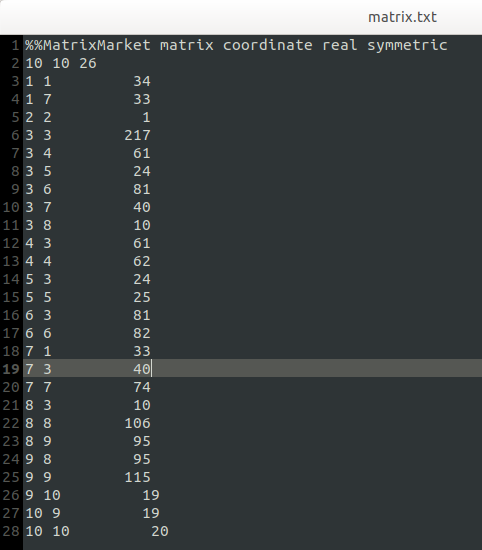
\includegraphics[scale=0.8]{matrix_example.png}
\end{center}
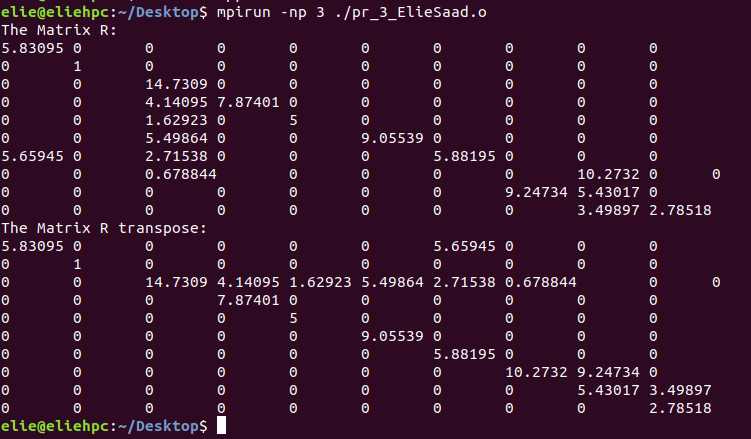
\includegraphics[scale=0.8]{matrix_calculation_output.png}

\pagebreak

\begin{thebibliography}{9}
\expandafter\ifx\csname natexlab\endcsname\relax\def\natexlab#1{#1}\fi
\expandafter\ifx\csname url\endcsname\relax
  \def\url#1{{\tt #1}}\fi

\bibitem{sympd}
Massachusetts Institute of Technology.
\newblock Symmetric matrices and positive definiteness.
\newblock Fall 2011.
\newblock URL \url{https://ocw.mit.edu/courses/mathematics/18-06sc-linear-algebra-fall-2011/positive-definite-matrices-and-applications/symmetric-matrices-and-positive-definiteness/MIT18\_06SCF11\_Ses3.1sum.pdf}.
\newblock [20/4/2020], pages 1 -- 2.

\bibitem{positivedefinite}
D. Kincaid and W. Cheney.
\newblock Numerical Analysis: Mathematics of Scientific Computing.
\newblock 3rd Edition, (American Mathematical Society, Providence, RI, 2002), page 145.
  
\bibitem{golub83matrix}
G.~H. Golub and C.~F. {Van Loan}.
\newblock {\em Matrix Computations}.
\newblock Johns Hopkins University Press, 1996.

\bibitem{preconditioners}
Massachusetts Institute of Technology.
\newblock {\em Lec 15 | MIT 18.086 Mathematical Methods for Engineers II}.
\newblock URL \url{https://www.youtube.com/watch?v=LtNVodIs1dI&t=764s}.
\newblock time 2:00 -- 13:32.
\end{thebibliography}

\end{document}